\documentclass[12pt]{article}
\usepackage{graphicx}
\usepackage[a4paper, total={6in, 9in}]{geometry}

\title{Projet bataille navale pour interface graphique}
\author{Abdulaziz Kalash,
Feras Makhlouf,
Mahmoud Harrak,
Tariq Abdulrazak}

\date{\today}

\begin{document}

\maketitle 
\begin{figure}[h]
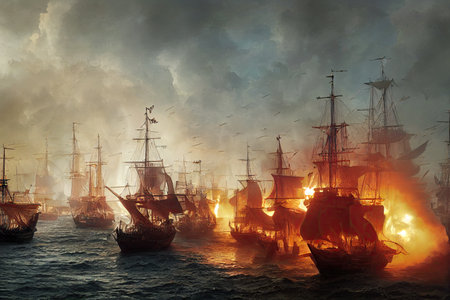
\includegraphics[scale=1.2]{bateau.jpg}
\end{figure}
\newpage
\tableofcontents 

\newpage 

\section{Introduction}

\subsection{Présentation du projet}
La bataille navale est un jeu de société bien connu qui a été popularisé au 20ème siècle. Le but du jeu est de localiser et de couler les navires de l'adversaire en lançant des missiles sur une grille de jeu. C'est un jeu simple mais amusant qui peut être joué par des joueurs de tous âges.
Dans le cadre de ce projet, nous avons entrepris de développer une version informatisée de la bataille navale en utilisant Java. L'objectif était de créer une application conviviale et fonctionnelle qui permettrait aux utilisateurs de jouer à la bataille navale contre un adversaire informatique (cet adversaire joue aléatoirement).
\subsection{Objectifs du projet}
Le projet avait plusieurs objectifs clés. Tout d'abord, nous souhaitions concevoir une interface utilisateur intuitive et facile à utiliser qui permettrait aux utilisateurs de jouer à la bataille navale sans difficulté. 
Mais tout cela en gardant le principe de MVC(modèle vue contrôleur), autrement dit, notre jeu reste complètement jouable en ligne de commande et le faite d'ajouter une interface graphique ne change absolument rien à notre code du modèle.
Nous avons également cherché à généraliser le plus possible, c'est-à-dire que notre code marche pour n'importe quelle taille de grille (tant qu'elle est carrée).
Enfin, nous avons cherché à concevoir l'application de manière à ce qu'elle soit extensible et facile à maintenir, de sorte que des améliorations puissent être apportées à l'avenir sans avoir à repenser complètement le code.

\subsection{Contexte}
Le projet a été réalisé dans le cadre de 4 cours d'interface graphique, qui visaient à nous donner une expérience pratique de la conception et du développement de logiciels en équipe. Nous avons travaillé ensemble pour identifier les exigences du projet, élaborer un plan de travail et mettre en œuvre des solutions techniques pour surmonter les défis rencontrés tout au long du développement 

Au-delà de la simple programmation, le projet nous a permis de développer nos compétences en matière de gestion de projet, de communication d'équipe et de résolution de problèmes. Nous avons travaillé en étroite collaboration pour assurer que le développement se déroule sans accroc et que l'application soit livrée à temps pour la date limite fixée (15/04/2023).
\newpage 

\section{Description de la bataille navale}

\subsection{Règles du jeu}
La bataille navale est un jeu de société pour deux joueurs, où chacun dispose d'une grille sur laquelle il place ses bateaux de différentes tailles. Le but du jeu est de couler tous les bateaux de l'adversaire en lançant des tirs sur sa grille. Les joueurs alternent les tours en essayant de toucher les cases de la grille de l'adversaire où se trouvent les bateaux. Si un bateau est touché sur une case, le joueur annonce "touché". Si toutes les cases du bateau sont touchées, le joueur annonce "coulé". Le premier joueur à couler tous les bateaux de l'adversaire remporte la partie.

\subsection{spécificités de nos règles}
Voici les spécificités des règles que nous avons implémentées dans notre jeu de bataille navale :
\begin{itemize}
    \item La grille peut avoir n'importe quelle taille (tant qu'elle est carrée).
    \item Le nombre de bateaux dans chaque grille dépend seulement de la taille de la grille, cette taille est la moitié de la longueur de l'axe des x (exemple : 5 bateau pour une grille de 10 x 10)
    \item La taille des bateaux ne sont pas définit à l'avance, pour chaque partie on tire n taille différente dans l'intervalle [taille min, taille max],
avec n : le nombre totale de bateaux,
	 taille min : la taille minimale d'un bateau (longueur axe des x / 5),
	 taille max : la taille maximale d'un bateau (longueur axe des x / 2).
	\item Les deux joueurs ont les mêmes bateaux, c'est-à-dire que c'est le même tirage pour les deux, si on tire le tableau [3,4,5,2,3] pour une grille de taille 10 x 10, alors ceci veut dire que nous allons avoir 5 bateaux (car taille du tableau) et que nous avons deux bateaux de taille 3, un bateau de taille 4, un bateau de taille 5 et un bateau de taille 2
	
	\item L'emplacement des bateaux n'est pas décidé par le joueur, c'est fait aléatoirement pour les deux !
	
\end{itemize}

Pour résumer, dans nos règles, quand une grille est plus grande le nombre de bateaux pour chaque joueurs et les tailles des bateaux augmentent.
\newpage 

\section{Conception du projet}


\subsection{Analyse des besoins}
Avant de commencer à concevoir l'application, nous avons d'abord effectué une analyse approfondie des exigences du projet. Nous avons identifié les fonctionnalités clés dont l'application avait besoin, telles que un projet 100% MVC avec d'abord un jeu sans interface graphique, puis l'ajout de l'interface graphique sans changer le code de notre jeu.

Nous avons également pris en compte les contraintes techniques du projet, notamment les langages de programmation et les outils disponibles pour développer l'application, ainsi que les délais impartis pour le développement et la livraison de l'application.

\subsection{Choix des technologies}
Nous devions utiliser le langage de programmation Java pour développer l'application. Nous avons également utilisé la bibliothèque graphique Swing pour la conception de l'interface utilisateur, car elle offre une grande flexibilité et est facile à utiliser.

Nous avons en majorité utilisé vsCode pour l'éditeur, car nous trouvons que c'est beaucoup plus utile pour nous en tant que étudiants, surtout que les éditeurs comme eclipse font eux seules une bonne partie du travail à notre place.

Nous avons utilisé Git pour le contrôle de version du code source et la forge pour héberger le projet et faciliter la collaboration entre les membres de l'équipe.

\subsection{Architecture du projet}

Nous avons conçu l'application en utilisant une architecture de modèle-vue-contrôleur (MVC). Cette architecture permet de séparer la logique métier de la présentation de l'interface utilisateur, ce qui facilite la maintenance du code et permet d'ajouter de nouvelles fonctionnalités plus facilement à l'avenir.

Le modèle représentait l'état actuel du jeu, y compris les positions des navires et les coups joués par les joueurs. Le contrôleur était responsable de la gestion des actions des utilisateurs, comme les coups joués, tandis que la vue représentait l'interface utilisateur de l'application.



\newpage
\begin{figure}[h]
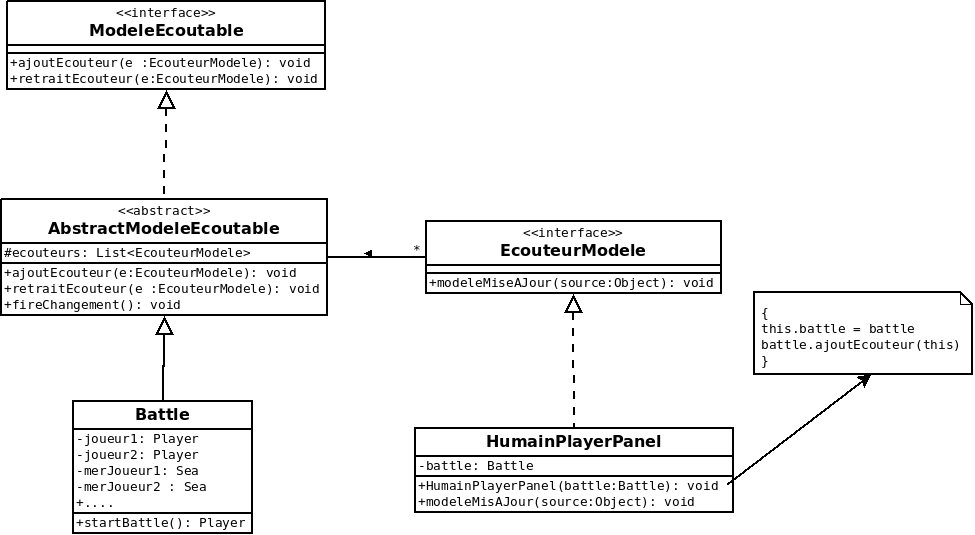
\includegraphics[scale=0.5]{Diagramme1.png}
\caption{Diagramme de classe mvc}
\end{figure}

Pour la construction mvc nous avons une classe abstraite \textbf{AbstractModeleEcoutable} qui va représenter tous les modèle qui l'ont peut écouter, cette classe possède 3 méthodes, deux parmis elles pour ajouter ou retirer un \textbf{EcouteurModele} et la dernière pour avertir tous les \textbf{EcouteurModele} que le modèle a changé, notre classe \textbf{Battle} est un \textbf{AbstractModeleEcoutable} donc elle possède la méthode fireChangement() qu'on appelle à chaque tour de boucle de jeu.

De l'autre coté, l'interface \textbf{EcouteurModele} représente toutes les vues, autrement dit, toutes les classes qui vont pouvoir écouter une autre classe, cette interface possède une méthode abstraite ModeleMiseAJour() qui est appelé à chaque fois que le modèle appelle la méthode fireChangement(), cette méthode ModeleMiseAJour() dit à notre affichage qu'il doit se mettre à jour car le modèle a changé.

Ici \textbf{HumainPlayerPanel} est un JPanel qui contient tout simplement la grille, car dans les mise à jour c'est seulement la grille qui change.
Dans notre \textbf{HumainPlayerPanel} nous avons une instance de notre modèle et donc on appelle la méthode ajoutEcouteur() dans la vue elle même, comme ceci on évite de changer le code de notre modèle à chaque fois que l'ont veut ajouter une vue.

\newpage	

\subsubsection{Les packages}
Nous avons séparé le code en plusieurs package et voici leurs utilités :

\begin{itemize}

\item \textbf{sea} : c'est dans ce package que l'on retrouve la conception de la notions de la mer (grille de jeu), ce package contient deux classes, \textbf{SeaCell} une classe qui représente une cellules de la mer, cette cellules possède plusieurs états, elle peut être détruite ou pas et elle peut contenir un bateau ou pas.

La classe \textbf{Sea} représente la grille d'un joueur, cette grille est composé de SeaCell, c'est dans cette classe qu'on associe a un joueur donnée, ses bateaux.

\item \textbf{players} : c'est un package dans lequel on retrouve tout les types de joueurs, on a par exemple le joueur "bot" qui va être l'adversaire à chaque partie (ce joueurs tire ses coups au hasard), on a aussi le joueur clavier qui lui va tirer sur une position a l'aide du terminale et de son clavier et finalement le joueur GUI qui lui tire en choisissant la position sur l'interface graphique.

De plus, chaque joueur possède une méthode d'affichage de l'état actuel du jeu, par exemple le joueur bot n'a pas d'affichage car cela ne sert à rien, le joueur GUI son affichage se fait sur l'interface graphique, et le joueur clavier il a un affichage dans le terminale.

\item \textbf{boat} : Dans le package boat on retrouve tout ce qui est en rapport avec les bateaux, par exemple les tailles minimale et maximale pour un bateau, toutes les vérifications pour savoir si un bateau est bien placé ou pas et toutes les informations d'un bateau donné.

Dans notre projet un bateau est une liste de cellules, cette liste n'a pas de contrainte au début, mais un bateau ne peut pas être construit s'il ne respecte pas certaines contraintes, par exemples, les cellules de ce bateaux doivent se suivre dans un seul sens, les cellules de ce bateau ne doivent ni être détruite (lors de la construction du bateau) ni contenir un autre bateau, le nombre de cellules de ce bateau doivent respecter l'intervalle [taille min, taille max].

Si un bateau respecte tout cela alors il est construit, sinon on le construit même pas, c'est pourquoi dans notre classe Sea nous avons pas besoin de vérifier si les bateau sont bien placé, car si par malheur ils ne le sont pas, alors ils ne seront même pas construit.

\item \textbf{generateur} : C'est un package qui contient une Classe \textbf{Generateur}, cette classe crée deux grille pour deux joueurs donnée, elle crée aussi n bateaux pour chaque grilles et elle place les bateaux. 

\item \textbf{battle} : Ce package contient les deux classes exécutable de notre projet, \textbf{MainClavier} et \textbf{MainGUI} comme leurs noms l'indiquent l'une est pour jouer dans le terminale avec l'affichage terminale et l'autre pour jouer sur l'interface graphique.

Dans ce package nous avons aussi la classe \textbf{Battle}  qui représente notre modèle, cette classe possède une méthode startBattle() qui commence le jeu entre les deux joueurs.

\item \textbf{graphique} : C'est un package qui contient tout ce qu'est lié avec la partie graphique de notre projet, nous allons revenir dessus plus tard.


\end{itemize}


\subsection{Partie graphique}

\subsubsection{Généralité}

Pour factoriser au mieux le code des grilles nous avons décidé d'avoir une seule classe qui va représenté la grille du joueur actuel et la grille de l'ennemie.

Cette classe contient une grille de boutons, ces boutons peuvent changer de couleur de fond dans le cas ou la case qui correspond au bouton est détruite, ils peuvent aussi avoir des bordure en fonction de s'ils contiennent des bateaux ou pas.

Notre fenêtre (JFrame) contient deux grille, à droite la grille du bot qui choisit des cases au hasard et à gauche la grille du joueur, quand une case est détruite et qu'elle ne contient pas de bateau alors elle est en vert, quand une case est détruite et qu'elle contient un bateau elle est en rouge, quand un bateau ennemi est complètement détruit on ajoute des bordures  et nos bateaux qui sont sur la grille adverse sont visible dés le début.

\subsubsection{GameButton}
GameButton est une classe abstraite qui représente les boutons de nos grilles, cette classe possède un attribut cellule qui représente la cellule que ce bouton est censé représenté, donc la couleur et les bordures du bouton changent en fonction de l'état de la cellule.
Cette classe extends JButton et met la couleur de fond à bleu par défaut, cette classe possède deux méthode, une méthode concrète update() qui va mettre à jour la couleur du fond de notre grille (concrète car c'est le même traitement pour les deux types de boutons) et une méthode abstraite personalUpdate() qui va gérer les bordure, elle est abstraite car la gestion de bordure dépend du type du bouton, si le bouton est dans la grille du joueur, alors les bordure sont affiché qu'une fois que le bateau est coulé, alors que sur la grille du bot, on les affiche dés le début.


\subsubsection{GameButtonB}
 La classe GameButtonB étend GameButton et représente un bouton pour
 l'affichage de la grille de l'adversaire (ma grille sur la quelle
 l'adversaire joue)
  qui contient un bateau. Elle gère également la bordure du bouton pour
 représenter le bateau de manière plus
  visuelle.
 Les bateaux sont affiché dès le début.


\subsubsection{GameButtonH}
  La classe GameButtonH hérite de la classe GameButton et représente un bouton
  de la grille de jeu pour les bateaux détruits.
  
  Elle permet de personnaliser l'apparence du bouton en fonction de l'état du
  bateau qui occupe la cellule associée.
  
  Les bateaux sont affiché qu'une fois qu'ils sont détruit, autrement dit c'est
  les boutons de la grille du bot(c'est la grille sur
  laquelle l'utilisateur joue)
  

\subsubsection{Séparation}

La séparation se fait lors de la création de la grille, nous avons un boolean qui nous indique si cette grille doit contenir des GameButtonH ou pas

\begin{figure}[h]
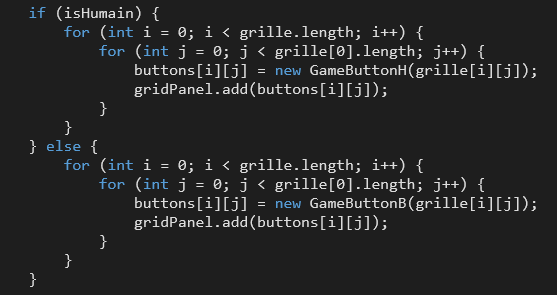
\includegraphics[scale=1.2]{code.png}
\caption{Séparation des boutons}
\end{figure}


Si le joueur est humain alors on remplit la grille de GameButtonH sinon on la remplit de GameButtonB, comme ceci nous gardon la même classe pour la grille c'est juste le type des bouton qui changent.


\subsubsection{Contrôleur}
Pour le contrôleur c'est simple, on ajoute un écouteur seulement sur les boutons de type GameButtonH, car si on clique sur la grille ennemi cela ne devrait rien changé, tout d'abord on vérifie si c'est autour du joueur humain de jouer, si ce n'est pas le cas on ne fait rien, sinon on vérifie si la cellule qui correspond au bouton cliqué n'est pas détruite, dans ce cas, on ne fait rien, si elle n'est pas détruite alors on la détruit.

\newpage

\section{Conclusion}

\subsection{Résumé du projet}
Dans l'ensemble, le projet de bataille navale en Java a été un succès. Nous avons réussi à concevoir et à développer une application fonctionnelle qui permet aux utilisateurs de jouer à la bataille navale. Nous avons également travaillé en étroite collaboration pour gérer le projet et surmonter les défis rencontrés tout au long du développement.
\subsection{Perspectives d'amélioration}
Cependant, il y a toujours des perspectives d'amélioration pour notre application. Par exemple, nous pourrions envisager d'ajouter des fonctionnalités telles que la possibilité de jouer avec une intelligence artificielle stratégique et la possibilité de suivre la progression à travers des scores et des parties enregistrées. Nous pourrions également améliorer l'interface utilisateur pour la rendre plus attrayante et conviviale.

Dans l'ensemble, nous sommes fiers du travail accompli et des compétences que nous avons acquises tout au long de ce projet. Nous sommes impatients de poursuivre notre apprentissage et de continuer à améliorer nos compétences en programmation et en développement de logiciels.

\end{document}
